\documentclass[11pt, oneside]{article}   	% use "amsart" instead of "article" for AMSLaTeX format
\usepackage{geometry}                		% See geometry.pdf to learn the layout options. There are lots.
\geometry{letterpaper}                   		% ... or a4paper or a5paper or ... 
%\geometry{landscape}                		% Activate for for rotated page geometry
%\usepackage[parfill]{parskip}    		% Activate to begin paragraphs with an empty line rather than an indent
\usepackage{graphicx}				% Use pdf, png, jpg, or eps� with pdflatex; use eps in DVI mode
								% TeX will automatically convert eps --> pdf in pdflatex		
\usepackage{amssymb}
\usepackage{amsmath}
\usepackage{parskip}
\usepackage{color}
\usepackage{hyperref}

\title{Orthogonality of sine and cosine:  summary}
%\author{The Author}
%\section{}
%\subsection*{}
\date{}							% Activate to display a given date or no date

\graphicspath{{/Users/telliott_admin/Dropbox/Tex/png/}}
% \begin{center} 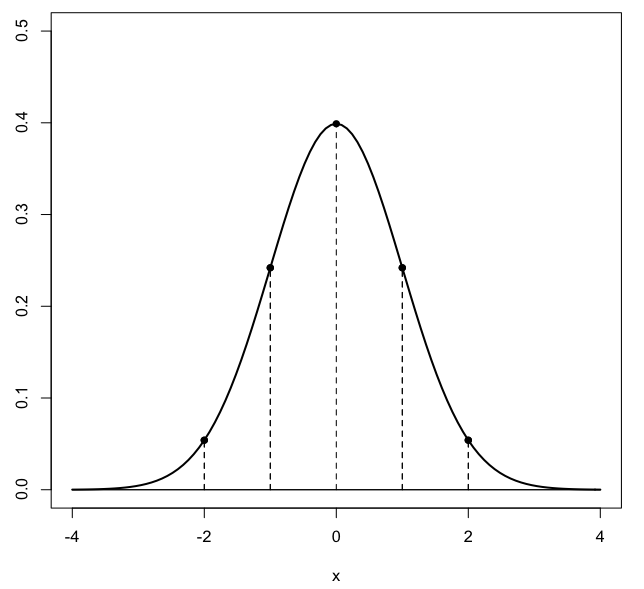
\includegraphics [scale=0.4] {gauss3.png} \end{center}
\begin{document}
\maketitle
\Large
This is a summary of the results for integrating products of sine and cosine in preparation for Fourier series.  In the derivation I did (elsewhere) I followed Paul in integrating $\int \cos n\pi x/L \cos m \pi x/L$ over $x = -L \rightarrow L$, etc.  

Other people do it more simply over the interval $x = -\pi \rightarrow \pi$, and obtain his results by a change of variable.  So here I will use the easier form.  See Wolfram for details about the change of variable.  As they say, for periodic $f(x)$ with period $2L$, any interval $[x_0, x_0 + 2L]$ will work.

\subsection*{cosine times cosine}
\[ \int_{-\pi}^{\pi} \cos mx \cos nx \ dx = \pi \delta_{mn} \]
$\delta_{mn}$ is the Kronecker delta:
\[ \delta_{mn} =  \ 
\begin{cases}
0 & n \ne m \\
1 & n = m \\
\end{cases} \]
I got this from Wolfram but actually it's not quite right.  If $n=m=0$ then the result should be $2\pi$.
\subsection*{sine times sine}
\[ \int_{-\pi}^{\pi} \sin mx \sin nx \ dx = \pi \delta_{mn} \]
\subsection*{sine times cosine}
\[ \int_{-\pi}^{\pi} \sin mx \cos nx \ dx = \frac{\sin^2}{2} \ \bigg |_{-\pi}^{\pi} = 0 \]
This is easy to prove.  For integer $k \in {0,\pm1,\pm2 \dots}$, the sine of $k\pi$ is zero.
Two other important results:
\[ \int_{-\pi}^{\pi} \sin nx  \ dx = 0 \]
\[ \int_{-\pi}^{\pi} \cos nx  \ dx = 0 \]

\subsection*{cofactors}
Let's write the formulas for the cofactors and then we'll look at how we got there.  The series for $f(x)$ is
\[ f(x) = \frac{1}{2}a_0 + \sum_{n=1}^{\infty} a_n \cos nx + \sum_{n=1}^{\infty} b_n \sin nx  \]
\[ a_0 = \frac{1}{\pi} \int_{-\pi}^{\pi} f(x) \ dx \]
\[ a_n = \frac{1}{\pi} \int_{-\pi}^{\pi} f(x) \cos nx \ dx \]
\[ b_n = \frac{1}{\pi} \int_{-\pi}^{\pi} f(x) \sin nx \  dx \]

\subsection*{evaluation}
To evaluate the cofactor $a_1$, multiply both sides by $dx$ and integrate term by term.  Every term like $\cos nx \ dx$ is really something else in disguise, namely
\[ \frac{1}{2\pi} \int_{-\pi}^{\pi} \cos nx \ \cos mx \ dx \]
with $m=0$!.  And as we saw, that integral is just $0$.  We are left with
\[ \frac{1}{2\pi} \int_{-\pi}^{\pi} f(x) \ dx = \frac{1}{2} \ a_0 \ \frac{1}{2\pi} \int_{-\pi}^{\pi} dx =  \frac{1}{2} \ a_0  \]
\[ a_0 = \frac{1}{\pi} \int_{-\pi}^{\pi} f(x) \ dx \]
All other terms like $a_1$ are found by multiplying the series by $\cos x$.  The only survivor is
\[ \frac{1}{2\pi} \int_{-\pi}^{\pi} f(x) \cos x \ dx = a_1 \ \frac{1}{2\pi} \int_{-\pi}^{\pi} \cos^2 x dx =  \frac{1}{2} \ a_1  \]
\[ a_1 = \frac{1}{\pi} \int_{-\pi}^{\pi} f(x) \cos x \ dx \]
\[ a_n = \frac{1}{\pi} \int_{-\pi}^{\pi} f(x) \cos nx \ dx \]
\[ b_n = \frac{1}{\pi} \int_{-\pi}^{\pi} f(x) \sin nx \ dx \]


\end{document}  